%------------------------------------------------------------------------------------------------------------------------
\chapter{序論}
\label{sec:josho}
%------------------------------------------------------------------------------------------------------------------------

フランスとスイスの国境にある欧州原子力研究機構 (CERN) に設置されている大型陽子衝突型加速器 (LHC) では、現在、素粒子物理学の基礎となっている標準模型の精密測定や標準模型を超える物理現象の探索が行われている。 ATLAS実験はLHC上にある4つの衝突点の1つで行われている実験であり、ATLAS 検出器を用いて 生成粒子の測定が行われている。LHCでは加速器のアップグレード(HL-LHC)を予定しており、これに向けてATLAS検出器のアップグレードを行う。本章ではLHC-ATLAS実験とそのアップグレード計画について説明する。



%------------------------------------------------------------------------------------------------------------------------
\section{素粒子標準模型 \cite{soryuushi}}
\label{sec:soryuushi}
%------------------------------------------------------------------------------------------------------------------------
物質を構成する最小の粒子は「素粒子」である。素粒子物理学を通して、自然界に存在する粒子やそれらの粒子がどのように相互作用するかを理解することができる。

現在、素粒子物理を考える枠組みとして、標準模型(SM: \textbf{S}tandard \textbf{M}odel)がある。標準模型は1970年代に確立された理論であり、2012年のHiggs粒子の発見を最後に、標準模型から予測される粒子が全て揃った。

本説では、標準模型の概要と、標準模型からは説明できない理論について説明する。


%------------------------------------------------------------------------------------------------------------------------
\subsection{標準模型の概要}
\label{sec:sm}
%------------------------------------------------------------------------------------------------------------------------

宇宙に存在する全てのものは、素粒子と呼ばれる17種類の粒子から構成され、4つの相互作用(電磁相互作用、強い相互作用、弱い相互作用、重力相互作用)により記述されている。\tref{tab:fermion}、\tref{tab:boson}に標準模型に登場する素粒子を示す。

%素粒子物理における粒子はスピンにより分類することができ、整数から$1/2$だけずれた値のスピンを持つ粒子をフェルミオン、整数値のスピンを持つ粒子をボソンと呼ぶ。

\begin{table}[htbp]
  \begin{center}
    \caption[標準模型での物質の構成粒子]{標準模型での物質の構成粒子}
    \label{tab:fermion}
    \begin{tabular}{|c||c|ccccl|}
    \hline
       & 世代 & 名称 & 表記 & 電荷$[\si{eV}]$ & スピン & 質量$[\si{GeV}]$ \\
    \bhline{1.5pt}
      \multirow{6}{*}{クォーク} & \multirow{2}{*}{第一世代}
           & アップクォーク & $u$ & $+2/3$ & $1/2$ & $2.3^{+0.7}_{-0.5} \times 10^{-3}$ \\
        &  & ダウンクォーク & $d$ & $-1/3$ & $1/2$ & $4.8^{+0.7}_{-0.3} \times 10^{-3}$  \\
        \cline{2-7}
        & \multirow{2}{*}{第二世代}
           & チャームクォーク & $c$ & $+2/3$ & $1/2$ & $1.275 \pm 0.025$ \\
        &  & ストレンジクォーク & $s$ & $-1/3$ & $1/2$ & $(95 \pm 5) \times 10^{-3}$  \\
        \cline{2-7}
        & \multirow{2}{*}{第三世代}
           & トップクォーク & $t$ & $+2/3$ & $1/2$ & $173.21 \pm 0.51 \pm 0.71$ \\
        &  & ボトムクォーク & $b$ & $-1/3$ & $1/2$ & $4.18 \pm 0.03$  \\
    \bhline{0.8pt}
      \multirow{6}{*}{レプトン} & \multirow{2}{*}{第一世代}
           & 電子ニュートリノ & $\nu_{e}$ & $0$ & $1/2$ & $< 1.1 \times 10^{-9}$ \\
        &  & 電子 & $e$ & $-1$ & $1/2$ & $0.511 \times 10^{-3}$  \\
        \cline{2-7}
        & \multirow{2}{*}{第二世代}
           & ミューニュートリノ & $\nu_{\mu}$ & $0$ & $1/2$ & $<0.19 \times 10^{-3}$ \\
        &  & ミューオン & $\mu$ & $-1$ & $1/2$ & $105.7 \times 10^{-3}$  \\
        \cline{2-7}
        & \multirow{2}{*}{第三世代}
           & タウニュートリノ & $\nu_{\tau}$ & $0$ & $1/2$ & $<18.2 \times 10^{-3}$ \\
        &  & タウ & $\tau$ & $-1$ & $1/2$ & $1777 \times 10^{-3}$  \\
    \hline
    \end{tabular}
  \end{center}
\end{table}

\begin{table}[htbp]
  \begin{center}
    \caption[標準模型での力を伝える粒子]{標準模型での力を伝える粒子}
    \label{tab:boson}
    \begin{tabular}{|c||l|cccll|}
    \hline
      & 名称 & 表記 & スピン & 電荷$[\si{e}]$ & 相互作用 & 質量$[\si{GeV}]$ \\
    \bhline{1.5pt}
      \multirow{4}{*}{ゲージボソン} & 光子 & $\gamma$ & 1 & 0 & 電磁相互作用 & $<1 \times 10^{-27}$ \\
      & W粒子 & $W^{\pm}$ & 1 & $\pm 1$ & 弱い相互作用 & $80.379 \pm 0.012$ \\
      & Z粒子 & $Z$ & 1 & 0 & 弱い相互作用 & $91.1876 \pm 0.0021$ \\
      & グルーオン & $g$ & 1 & 0 & 強い相互作用 & $0$ \\
    \bhline{0.8pt}
      スカラーボソン & ヒッグス粒子 & $H$ & 0 & 0 & 質量を与える & $125.7 \pm 0.4$ \\
    \hline
    \end{tabular}
  \end{center}
\end{table}


物質を構成する粒子はフェルミオンに分類される。フェルミオンとは整数から$1/2$だけずれた値のスピンを持つ粒子の総称であり、標準模型に含まれるフェルミオンは全て$1/2$のスピンを持つ。物質を構成する粒子は、強い相互作用をするかどうかでクォークとレプトンに分類される。
クォークは強い相互作用から自然界に単独で存在することができず、ハドロンというクォークの集合体で自然界に存在する。
3つのクォークから構成されるハドロンをバリオン、クォークとその反クォークのペアから構成されるハドロンをメソンと呼ぶ。
一方で、レプトンは強い相互作用の影響を受けないことから、単独で自然界に存在することができる。


力を媒介する粒子はボソンに分類される。ボソンとは整数値のスピンを持つ粒子の総称である。素粒子の間に働く力には、強い力、弱い力、電磁気力、重力の4種類があり、
標準模型では、強い相互作用、弱い相互作用、電磁相互作用が記述される。強い相互作用を記述する量子色力学(QCD: \textbf{Q}uantum \textbf{C}hromo\textbf{d}ynamics)と、弱い相互作用と電磁相互作用を記述するワインバーグ-サラム理論のゲージ場が組みとなり標準模型が導入され、3つの相互作用はスピン1のゲージボソンによって媒介される。

%ヒッグス
標準模型では、ゲージ場や基本粒子は質量を持たないものとしてラグランジアンの中に導入され、素粒子が質量を持つことはゲージ対称性の破れを表す。これは\tref{tab:fermion}、\tref{tab:boson}に示すように、素粒子が質量を持つことと矛盾する。そこで、対称性の破れを起こさせるヒッグス場の存在が提唱された。ヒッグス場は複素スカラー場で、その真空期待値$v\sim 250\ \si{GeV}$が対称性を破るとともに粒子に質量を与える。各粒子の質量は\fref{fig:higgs}のように、ヒッグス場との結合定数に比例する。ヒッグス場と粒子の間にあるの相互作用はスピン0のスカラーボソンであるヒッグス粒子によって媒介される。2012年のヒッグス粒子の発見\footnote{ヒッグス粒子はCERNのLHCで行われているATLAS実験とCMS実験で発見された。}を最後に、標準模型から予測される粒子が全て揃った。

\begin{figure}[tbp]
  \centering
  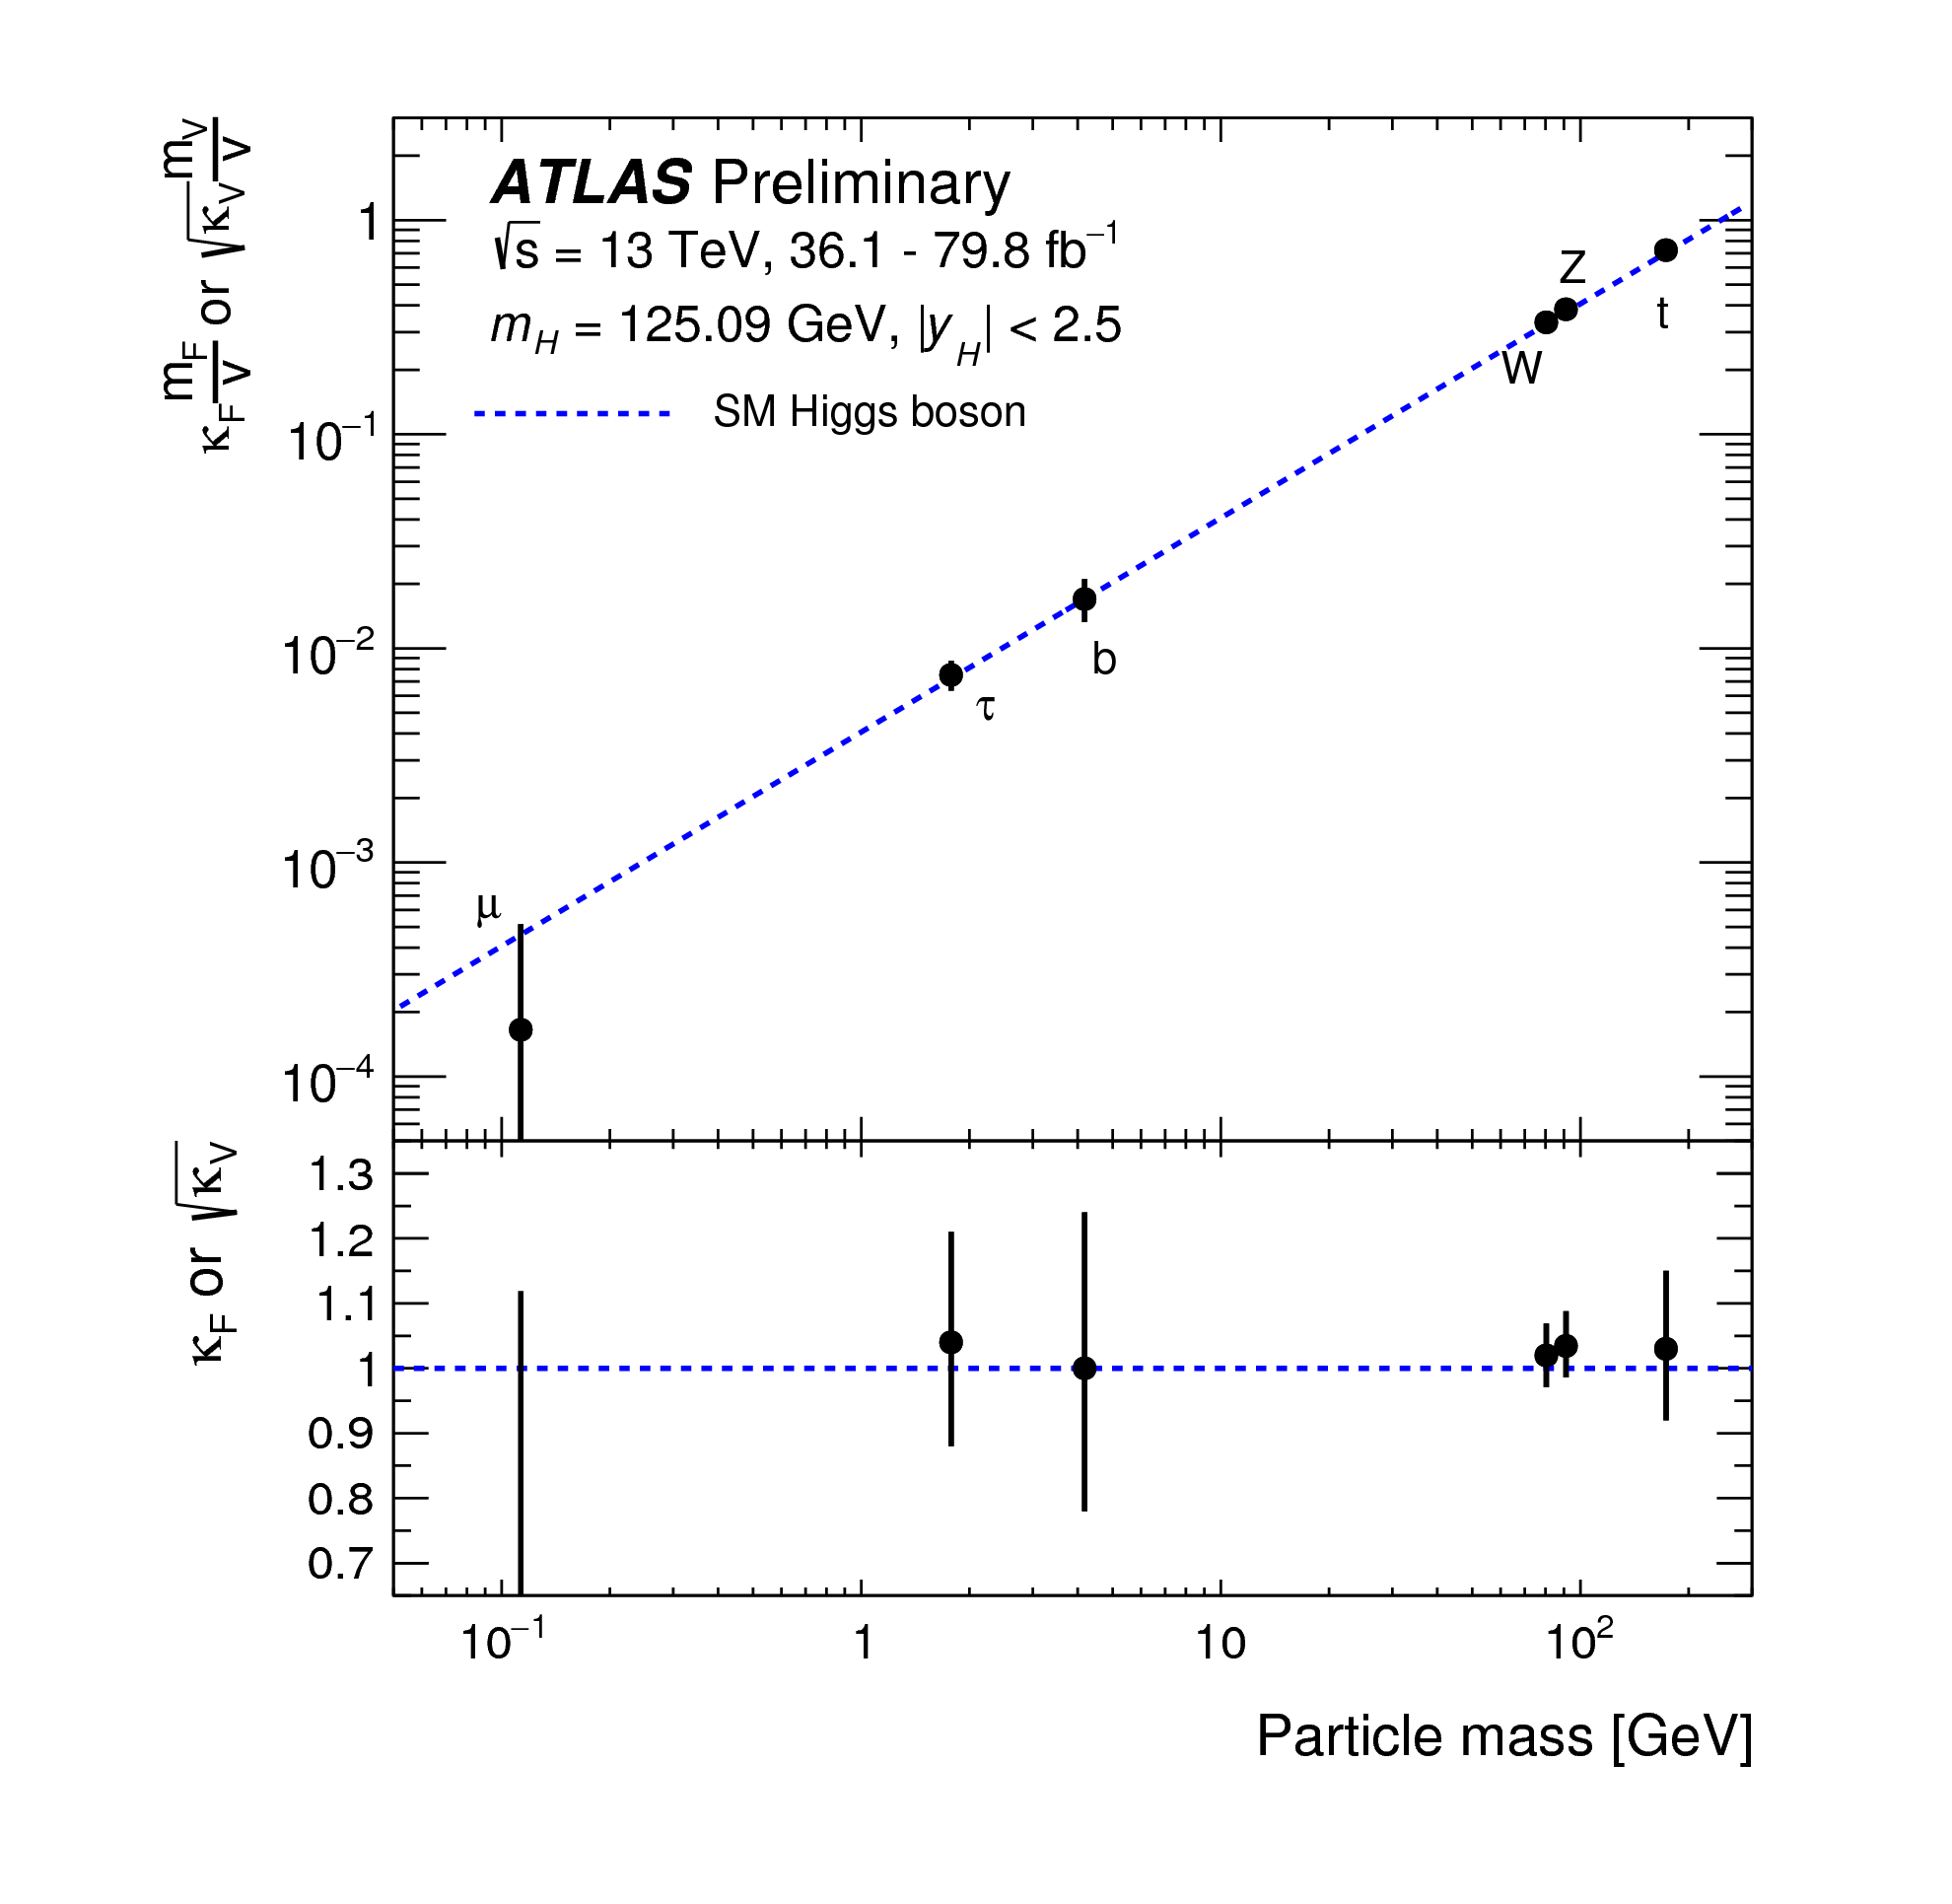
\includegraphics[height=9cm,keepaspectratio]{higgs.png}
  \caption[ヒッグス場との結合定数と素粒子の質量]{ヒッグス場との結合定数と素粒子の質量\cite{higgs}。$\kappa_\mathrm{F} m_\mathrm{F}/v$はフェルミオン($\mathrm{F}=t, b, \tau, \mu$)に対する結合定数を表し、$\kappa_\mathrm{F} m_\mathrm{F}/v$はボソン($\mathrm{V}=W, Z$)に対する結合定数を表す。$v$はヒッグス場の真空期待値を表す。 }
  \label{fig:higgs}
\end{figure}

%------------------------------------------------------------------------------------------------------------------------
\subsection{標準模型を超えた新物理の探索\cite{evidenceDark}}
\label{sec:bsm}
%------------------------------------------------------------------------------------------------------------------------

標準模型を用いて、これまでに行われた素粒子実験のほとんどの結果を矛盾なく説明することができる。しかし、標準模型では説明できない実験事実が確認されており、いくつかの点で不十分である。標準模型の問題の1つとして、暗黒物質が挙げられる。

暗黒物質が存在することの最も有力で直接的な実験事実は、銀河の回転曲線の測定から得られる。光学分光観測で得られる銀河全体の回転速度の分布は、銀河に含まれる星やガスから得られる物質分布から予想される回転速度よりもはるかに大きな回転速度が得られる。このことから、銀河には光学的な観測にかからない暗黒物質の存在が確認された。他にも、重力レンズ効果などの宇宙観測により、暗黒物質は宇宙全体のエネルギーの約$27\%$を占めることがわかっており、これは標準模型から得られる物質の約$6$倍の量に相当する。
暗黒物質の実態は未だわかっていないが、その候補としてWIMP(\textbf{W}eak \textbf{I}nteracting \textbf{M}assive \textbf{P}article)という、弱く相互作用する重くて安定な中性粒子が挙げられる。


暗黒物質の解明や、標準模型におけるその他の問題を解決するための新たな理論体系として、超対称性(SUSY: \textbf{Su}per \textbf{Sy}mmetry)理論がある。超対称性理論では、標準模型の全ての素粒子の対となり、スピンが$1/2$だけ異なる新たな素粒子が予言され、その中には暗黒物質の候補も含まれる。
\fref{fig:physics_bsm}に超対称性粒子と標準模型の素粒子の対応図を示す。
\begin{figure}[tbp]
  \centering
  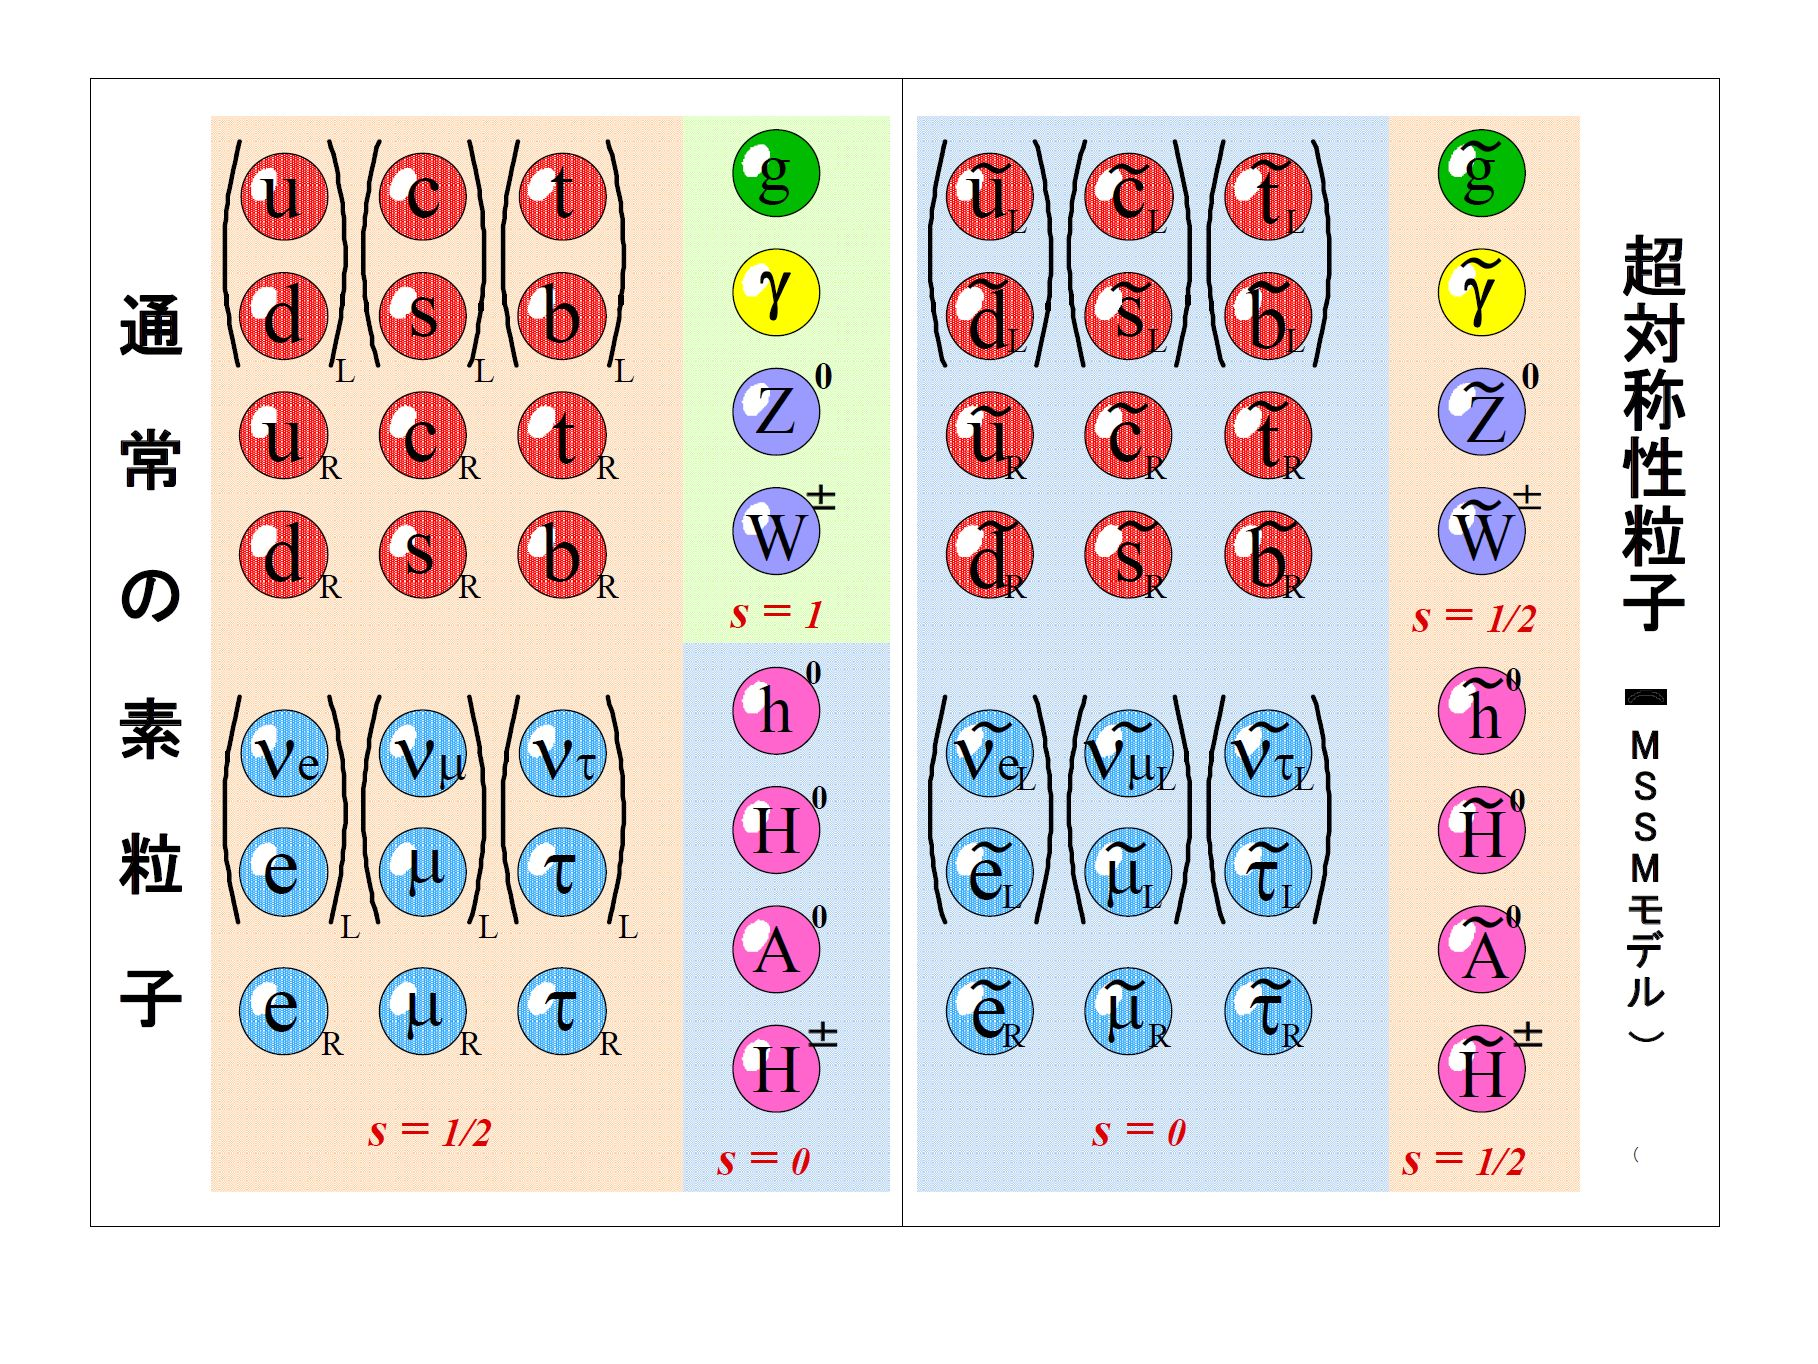
\includegraphics[height=8cm,keepaspectratio]{physics_bsm.jpg}
  \caption[超対称性粒子]{超対称性粒子 \cite{kek} }
  \label{fig:physics_bsm}
\end{figure}
超対称性粒子の中で最も軽いものをLSP(\textbf{L}ightest \textbf{S}USY \textbf{P}article)と呼ぶ。

超対称性理論は標準模型では説明が困難な問題を解決することができる一方で、バリオン数やレプトン数を破る相互作用の存在を避けることができない。バリオン数とレプトン数を破る現象のひとつとして陽子崩壊があるが、このような崩壊は観測されていない。この事実を説明するために、バリオン数とレプトン数を破る崩壊を禁止するRパリティを導入する。
Rパリティは\eref{eq:r}のように定義されている。
\begin{equation}
  \label{eq:r}
  R = (-1)^{3(B-L)}+2s
\end{equation}
ここで、$B, L$はそれぞれバリオン数、レプトン数であり、$s$はスピンである。Rパリティは標準模型の粒子では$1$となり、超対称性粒子では$-1$となる
Rパリティの保存から、標準模型の粒子と超対称性粒子に起こりうる崩壊は以下の3通りのみである。
\begin{itemize}
  \item $\mathrm{SM} \to \mathrm{SM} + \mathrm{SM}$
  \item $\mathrm{SM} \to \mathrm{SUSY} + \mathrm{SUSY}$
  \item $\mathrm{SUSY} \to \mathrm{SM} + \mathrm{SUSY}$
\end{itemize}
ここで、SMは標準模型の粒子、SUSYは超対称性粒子を表す。
超対称性粒子の中で最も軽いものであるLSP(\textbf{L}ightest \textbf{S}USY \textbf{P}article)はより軽い超対称性粒子が存在しないため、それ以上崩壊することができず安定な状態であることがわかる。したがって、中性のLSPはWIMPであり、暗黒物質の候補になりうる。
%また、重力レンズ効果等の他の宇宙観測からも暗黒物質の存在が確実視されている。


%\begin{figure}[tbp]
%  \centering
%  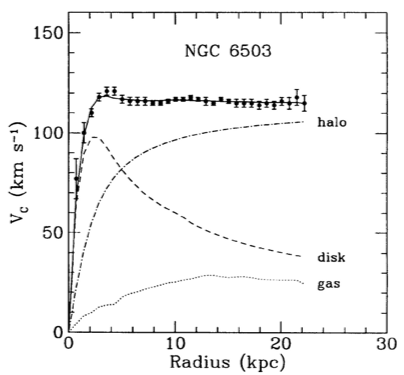
\includegraphics[height=7cm,keepaspectratio]{darkEvi.png}
%  \caption[NGC 6503 銀河の回転曲線]{ NGC 6503銀河の回転曲線 \cite{evidenceDark} }
%  \label{fig:physics_bsm}
%\end{figure}

他にも、超対称性理論の導入により、標準模型では説明できなかった問題が以下のように解決する。
\begin{itemize}
  \item 階層性問題の解決
  \item B/L対称性の破れの候補
  \item ニュートリノの質量形成のメカニズム
  \item 超ひも理論の特徴
\end{itemize}


%------------------------------------------------------------------------------------------------------------------------
\section{LHC}
\label{sec:LHC}
%------------------------------------------------------------------------------------------------------------------------

\begin{figure}[tbp]
  \centering
  \includegraphics[height=9cm,keepaspectratio]{LHC.jpg}
  \caption[LHCの全体図]{LHCの全体図 \cite{LHC} }
  \label{fig:LHC}
\end{figure}


LHC(\textbf{L}arge \textbf{H}adron \textbf{C}ollider)は欧州原子核研究機構(CERN)に建設された、周長がおよそ27\ \si{km}の陽子・陽子衝突型加速器である。陽子ビームの重心系エネルギーは世界最高のエネルギーである14\ \si{TeV}に到達できるよう設計されている。この世界最高のエネルギーを用いて、標準模型の精密測定やそれを超える新物理の探索がLHCの主な目的である。

\subsection{LHCの基本構造}
\fref{fig:LHC}にCERNに設置されている加速器・検出器の全体図を示す。陽子を生成し、加速器によって段階的に加速された2本の陽子ビームが、LHC周上において衝突する。


金属製の円筒に水素ガスを注入し、電場を用いて水素分子を陽子と電子に分離する。LHCのビームは、最大2808個のバンチと呼ばれる陽子のかたまりから構成され、$1.15\times 10^{11}$個の陽子が1バンチとして加速される。すなわち、LHCにおいて陽子陽子衝突から物理現象の探索をするためには、$2\ \mathrm{beams} \times 2808\ \mathrm{bunches}\times 1.15\cdot10^{11}\approx 6\cdot 10^{14}$個の陽子を生成する必要がある。

生成された陽子バンチは、初めに線形加速器 (LINAC\ 2)によって$50\ \si{MeV}$まで加速される。その後、陽子シンクロトロンブースター(PBS)、陽子シンクロトロン加速器(PS)、スーパーシンクロトロン加速器(SPS)によって段階的に$450\ \si{GeV}$まで加速され、2本の逆向きに加速された陽子バンチがLHCに投入される。LHCに投入された陽子バンチは$6.5\ \si{GeV}$(2018 年時点)まで加速されて、各衝突点において2つの陽子バンチが約$25\ \si{ns}$の間隔で衝突する。

LHCのビームパイプ上には4つの衝突点が設けられており、それぞれの衝突点において\ ATLAS(\textbf{A} \textbf{T}roidala \textbf{L}HC \textbf{A}pparata\textbf{S})、CMS(\textbf{C}ompact \textbf{M}uon \textbf{S}olenoid)、ALICE(\textbf{A} \textbf{L}arge \textbf{I}on \textbf{C}ollider \textbf{E}xperiment)、LHCb実験が行われている。




%------------------------------------------------------------------------------------------------------------------------
\subsection{ルミノシティ}
\label{sec:luminosity}
%------------------------------------------------------------------------------------------------------------------------

陽子ビームの強度を表すパラメータとして瞬間ルミノシティ$L$が用いられる。反応断面積$\sigma$の物理イベントが、1秒あたりに生じるイベント数 N は\eref{eq:lumi}で与えられる。
\begin{align}
  \label{eq:lumi}
  L = \gamma_{r} \frac{N_{b}^{2} n_{b} f_{rev}}{4\pi \varepsilon_{n} \beta^*}R
\end{align}
ここで、$N_{b}$は1バンチあたりに含まれる粒子数、$n_{b}$は1ビームに含まれるバンチ数、$f_{rev}$はビームの回転周波数、$\gamma_{r}$は陽子ビームのローレンツ因子、$\varepsilon_{n}$はビーム軸に垂直な平面でのビームの広がり、$\beta^{*}$は衝突点における振幅の大きさである。$R$は幾何学的損失係数という、ビーム衝突が有限の角度で起きることによる係数であり、\eref{eq:kikaf}で表される。
\begin{equation}
  \label{eq:kikaf}
  R=\left( 1+\left( \frac{\theta_{c}\sigma_{z}}{2\sigma^{*}} \right)^2 \right)^{-1/2}
\end{equation}
ここで、$\theta_c$は衝突時ビーム交差角、$\sigma_z$は衝突時におけるバンチ長の標準偏差、$\sigma^*$は衝突時におけるのバンチ幅の標準偏差である。

単位時間あたりに起こる物理事象の回数$N_\mathrm{event}$は、瞬間ルミノシティ$L$と反応断面積$\sigma$を用いて\eref{eq:hannnou}のように表すことができる。
\begin{equation}
  \label{eq:hannnou}
  N_\mathrm{event} = \int L\ dt\ \sigma
\end{equation}




%------------------------------------------------------------------------------------------------------------------------
\section{ATLAS実験}
\label{sec:ATLAS}
%------------------------------------------------------------------------------------------------------------------------
\begin{figure}[tbp]
  \centering
  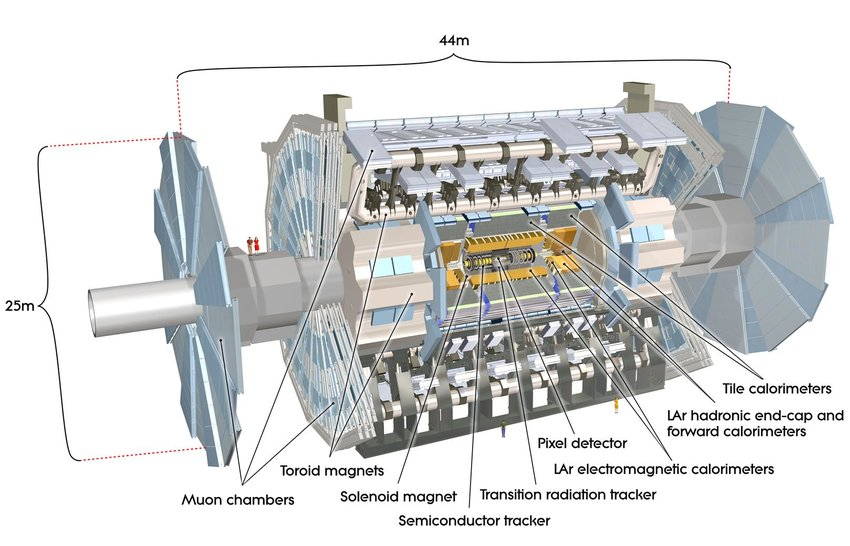
\includegraphics[height=7cm,keepaspectratio]{ATLAS.jpg}
  \caption[ATLAS検出器]{ATLAS検出器の全体図 \cite{ATLAS}。円筒の中心の内側から順に、内部飛跡検出器、電磁カロリメータ、ハドロンカロリ
  2 メータ、ミューオン検出器が衝突点を覆うように存在する。}
  \label{fig:ATLAS}
\end{figure}


ATLASはLHCの衝突点の一つに設置されている汎用型の検出器である。\fref{fig:ATLAS} に示すように、ATLAS検出器は直径25\ \si{m}長さ44\ \si{m}の円筒型をした巨大な検出器である。その中心に陽子の衝突点があり、LHCによって加速された陽子ビームが円筒の中心軸を通過するような構造になっている。
陽子ビームの衝突点である円筒の中心の内側から順に、内部飛跡検出器、電磁カロリメータ、ハドロンカロリメータ、ミューオン検出器が衝突点を覆うように存在する。内部飛跡検出器と電磁カロリメータの間にはソレノイド磁石、ハドロンカロリメータの外側にはトロイド磁石が配置されている。



%------------------------------------------------------------------------------------------------------------------------
\subsection{ATLAS実験で使用される座標系}
\label{sec:zahyoukei}
%------------------------------------------------------------------------------------------------------------------------
\begin{figure}[tbp]
  \centering
  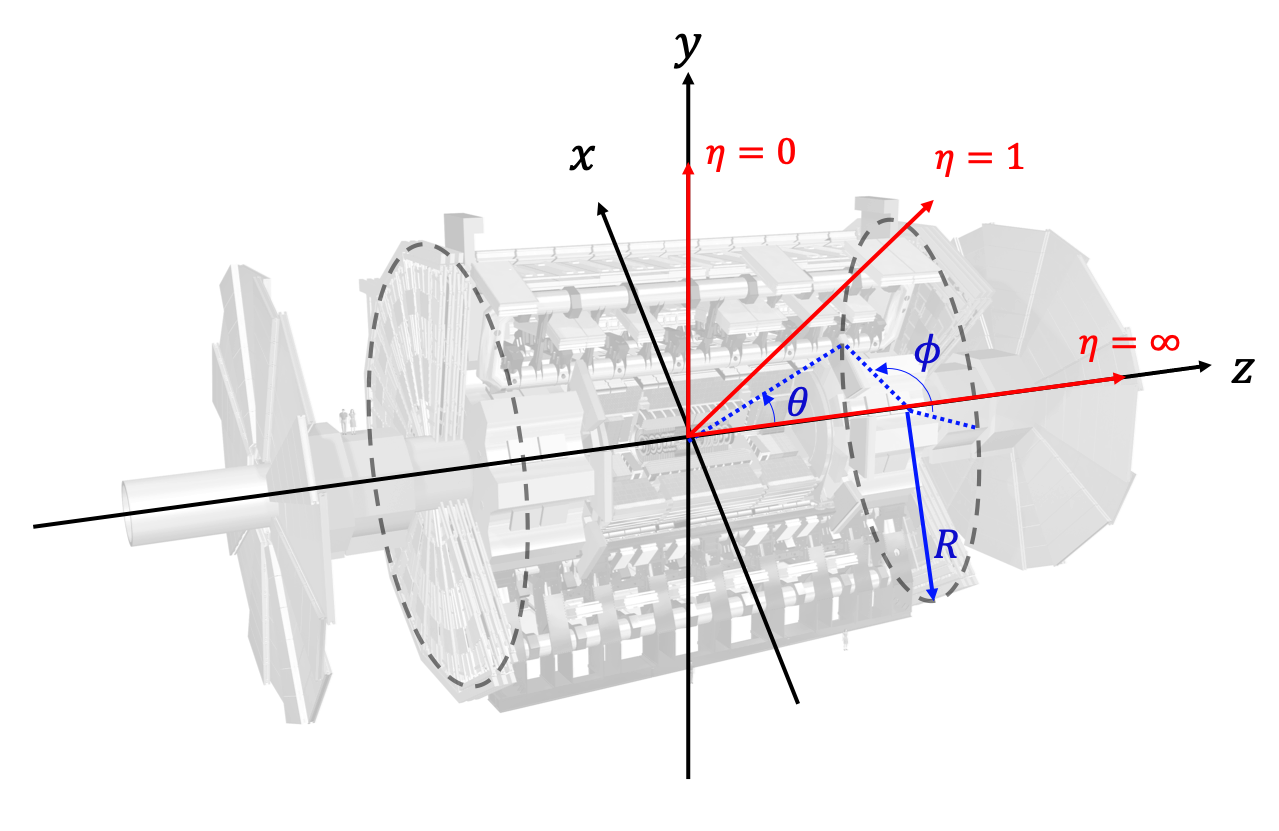
\includegraphics[height=7cm,keepaspectratio]{atlas_zahyou.png}
  \caption[ATLAS検出器]{ATLAS検出器で使用される座標系 \cite{ATLAS} }
  \label{fig:atlaszahyou}
\end{figure}

ATLASにおいて粒子の位置・運動量を示すために、\fref{fig:atlaszahyou}のような直交座標系$\left( x, y, z \right)$および円筒座標系$\left( R, \phi, z \right)$を用いる。直交座標系は陽子の衝突点を原点とし、LHCリングの中心方向を$x$軸、鉛直方向に上向きを$y$軸、ビーム軸を$z$軸と定義し、$z>0$はジュネーブ市内の方向を指す。$z$軸が正の領域をA-side、負の領域をC-sideと呼ぶ。
%\footnote{A-sideはAirportがある方向、C-sideはフランスの Saint-Genis-Pouilly という街にある Charly's Pub というバーがある方向}。
円筒座標系は$z$軸からの距離を$R$とし、$x\-y$平面内における方位角を$\phi$と定義する。また、$yz$平面における天頂角$\theta$を用いて擬ラピディティ(pesudorapidity) $\eta$を\eref{eq:eta}のように定義する。

\begin{equation}
  \label{eq:eta}
  \eta \equiv  -\ln\left( \tan{\left( \frac{\theta}{2} \right)} \right)
\end{equation}
擬ラピディティ$\eta$の差はローレンツ不変量であるため、ATLAS実験において粒子の位置や検出器の配置を示すために極角$\theta$ではなく擬ラピディティが用いられることが多い。$|\eta|$が小さくATLASの側面に対応する領域をバレル部、$|\eta|$が大きくATLASの底面に対応する部分をエンドキャップ部と呼ぶ。

%------------------------------------------------------------------------------------------------------------------------
\subsection{内部飛跡検出器}
\label{sec:InnerDetector}
%------------------------------------------------------------------------------------------------------------------------
\begin{figure}[tbp]
  \begin{minipage}[b]{0.45\linewidth}
    \centering
    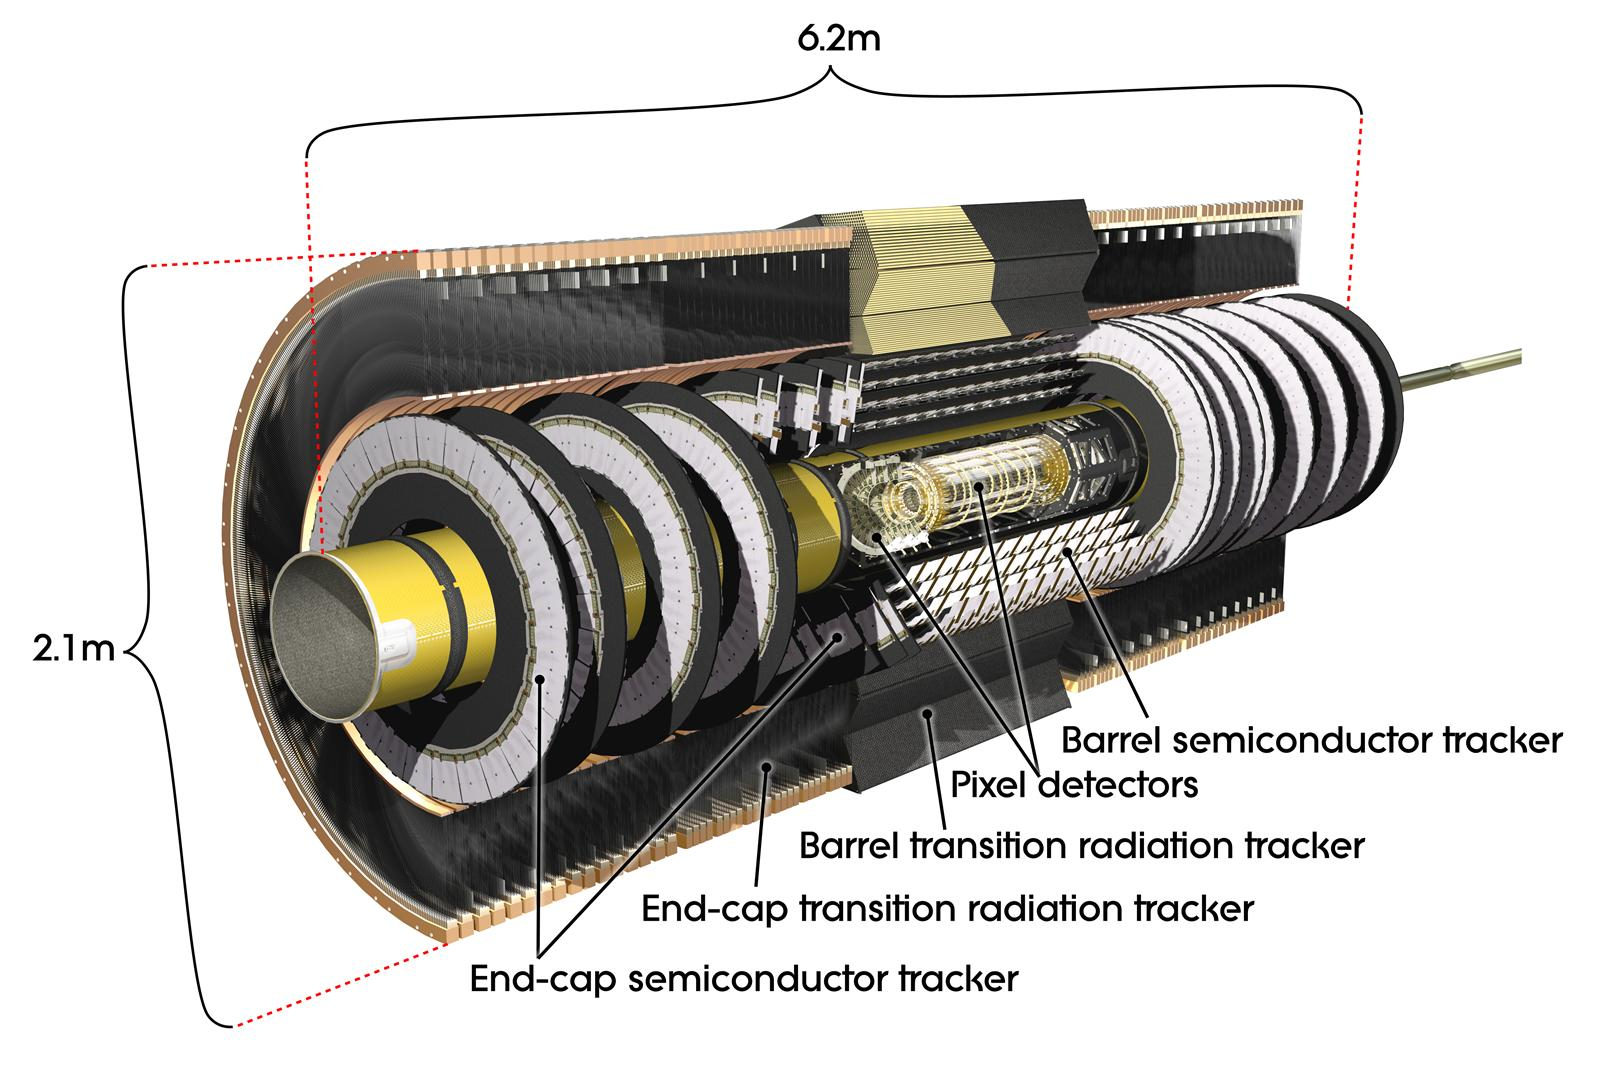
\includegraphics[keepaspectratio, scale=0.25]{InnerDetector.jpg}
    \caption{内部飛跡検出器の全体像。}
    \label{fig:InnerDetector}
  \end{minipage}
  \begin{minipage}[b]{0.45\linewidth}
    \centering
    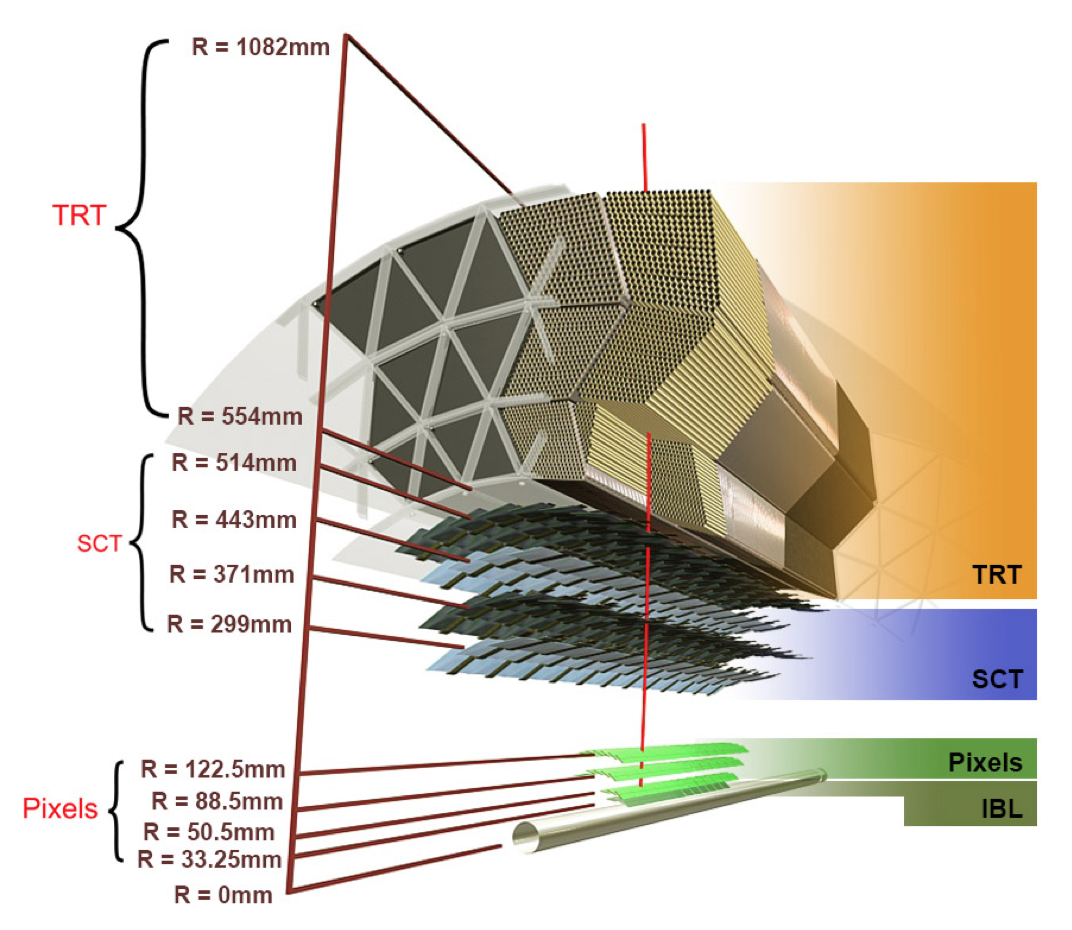
\includegraphics[keepaspectratio, scale=0.3]{structureID.png}
    \caption{内部飛跡検出器の断面図。}
    \label{fig:structureID}
  \end{minipage}
\end{figure}

\begin{figure}[tbp]
  \centering
  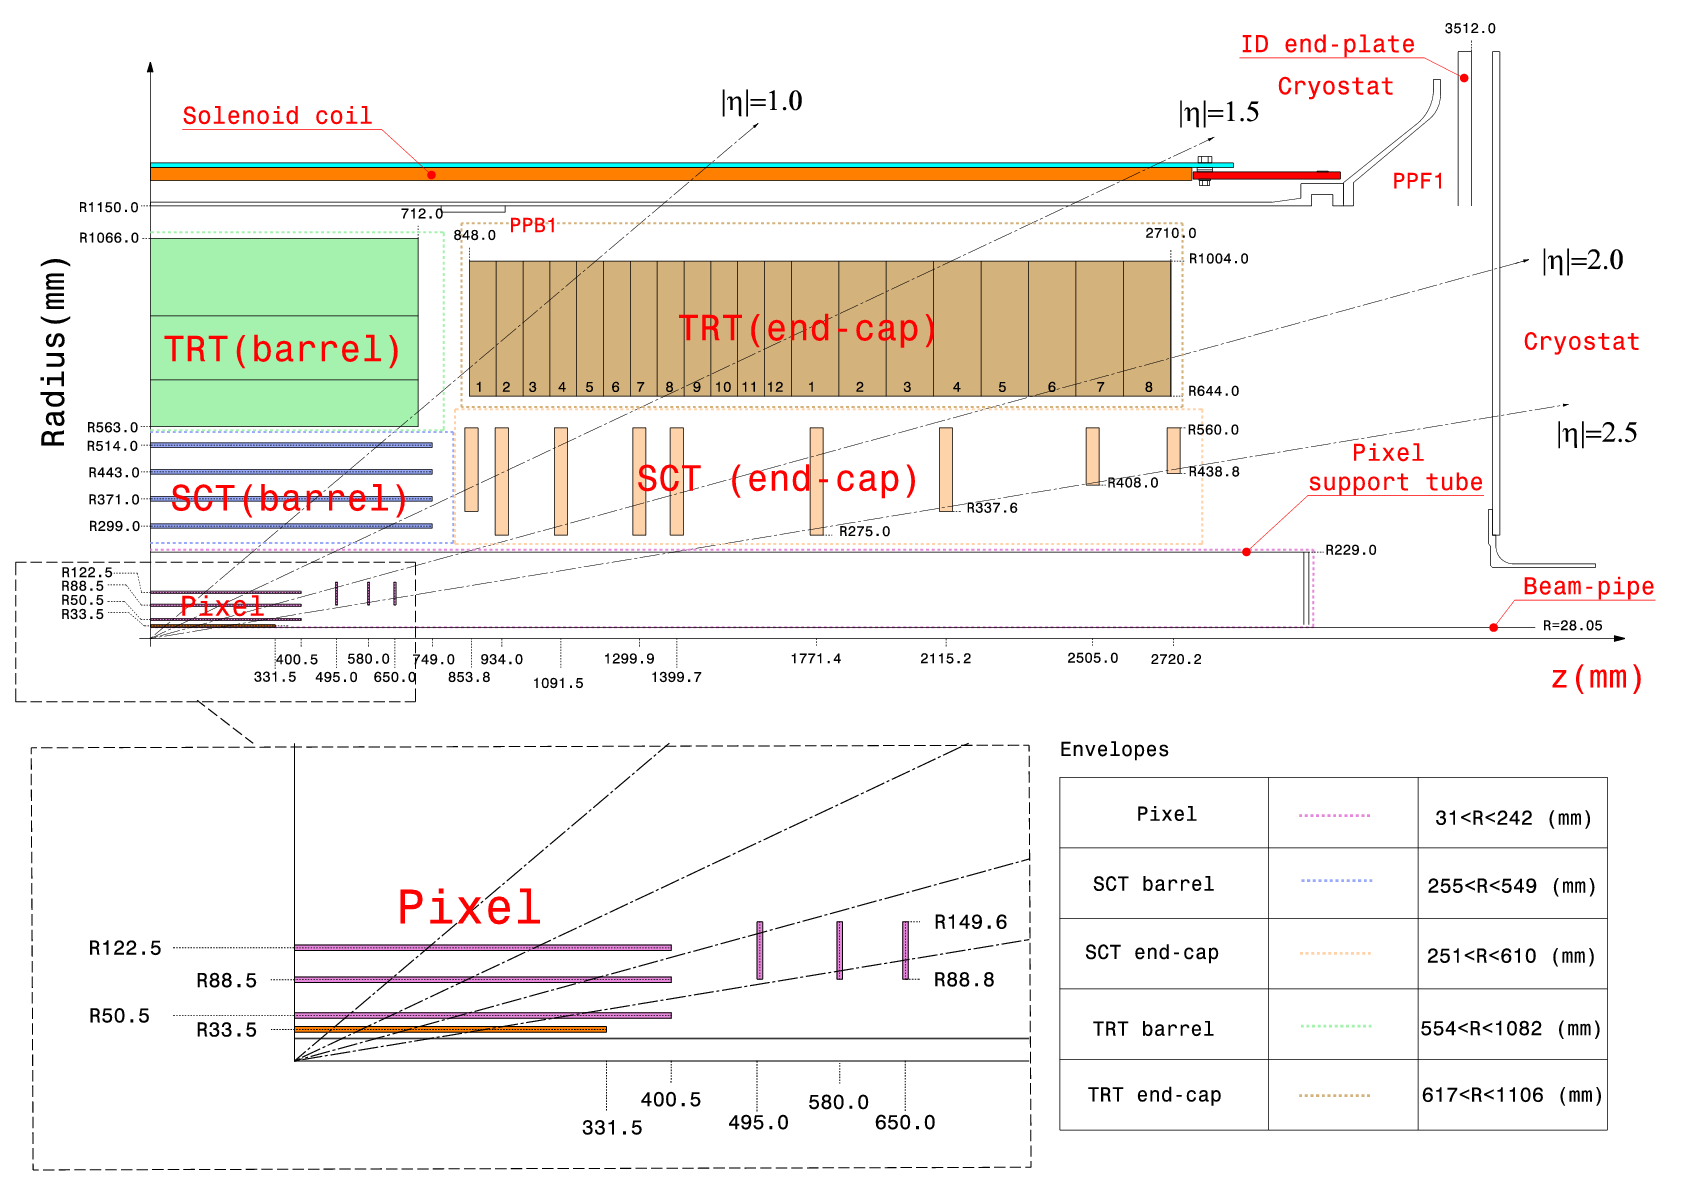
\includegraphics[height=7cm,keepaspectratio]{figures_final_pdf_NewID.png}
  \caption[内部飛跡検出器の配置]{内部飛跡検出器の配置 \cite{studyofID} }
  \label{fig:IDfigure}
\end{figure}


\fref{fig:InnerDetector}、\fref{fig:IDfigure}に内部飛跡検出器の全体図および断面図を示す。内部飛跡検出器はATLASの最内層に配置され、内側から順にIBL、ピクセル検出器、ストリップ検出器、遷移放射検出器で構成されている。衝突点から生成された荷電粒子を検出することで飛跡の再構成を行う。内部飛跡検出器の外側に配置されたソレノイド磁石により、$2\ \si{T}$の磁場がビーム軸に並行な方向にかけられる。


%------------------------------------------------------------------------------------------------------------------------
\subsubsection{IBL、ピクセル検出器}
\label{sec:pixels}
%------------------------------------------------------------------------------------------------------------------------

IBL(\textbf{I}nsertable \textbf{B}-\textbf{L}ayer)およびピクセル検出器はシリコン半導体検出器であり、内部飛跡検出器の最内層に配置されている。IBLはバレル部に1層配置され、ピクセル検出器はバレル部が3層、エンドキャップ部が片側3層で構成される。IBL、ピクセル検出器が配置を\tref{tab:pixel}に示す。

ピクセル検出器はLHCの運転開始時である2007年から稼働している検出器であり、読み出しチップにFE-I3という$50\times400\ \si{\micro m^2}$のピクセルを持つASICが使用されている。
IBLは、LHCにおける2年間のシャットダウン期間(2012年 - 2014年)に新たに設置された。IBLは陽子ビームの衝突点に最も近い検出器のため、高い放射線耐性と多い事象数を処理することができるように設計されている。読み出しチップにはFE-I4と呼ばれる、$50\times250\ \si{\micro m^2}$のピクセルを持つASICが使用されている。これらのASICの詳細については\ref{sec:genkoupixel}節に示す。

\begin{table}[htbp]
  \begin{center}
    \caption[IBL、ピクセル検出器の配置]{IBL、ピクセル検出器の配置}
    \label{tab:pixel}
    \begin{tabular}{|c||c|c|c|c|c|}
    \hline
       &  & $R\ [\si{mm}]$ & $z\ [\si{mm}]$ & 検出器の総数 & ピクセルの総数$(\times 10^{6})$ \\
    \bhline{1.5pt}
    \multirow{4}{*}{Barrel}
     & IBL & $33.5$ & $ < 331.5$ & $224$ & $6.02$ \\
     \cline{2-6}
     & B-layer & $50.5$ & $< 400.5$ & $286$ & $13.2$ \\
     \cline{2-6}
     & Layer 1 & $88.5$ & $< 400.5$ & $494$ & $22.8$ \\
     \cline{2-6}
     & Layer 2 & $122.5$ & $< 400.5$ & $676$ & $31.2$ \\
    \hline
    \multirow{3}{*}{Endcaps}
     & Disk 1 & $88.8 < R < 149.6$ & $495$ & $48\times2$ & $4.4$ \\
     \cline{2-6}
     & Disk 1 & $88.8 < R < 149.6$ & $580$ & $48\times2$ & $4.4$ \\
     \cline{2-6}
     & Disk 1 & $88.8 < R < 149.6$ & $650$ & $48\times2$ & $4.4$ \\
    \hline
    \end{tabular}
  \end{center}
\end{table}



%------------------------------------------------------------------------------------------------------------------------
\subsubsection{ストリップ検出器}
\label{sec:sct}
%------------------------------------------------------------------------------------------------------------------------
ストリップ検出器(SCT: \textbf{S}emi\textbf{C}onductor \textbf{T}racker)はシリコン半導体検出器であり、ピクセル検出器の外側に配置されている。バレル部4層で$|\eta|<1.4$の領域を、エンドキャップ部では片側9層ずつで$1.4<|\eta|<2.5$の領域を覆うように配置されている。
ストリップ検出器のモジュールはストリップが$80\ \si{\micro m}$間隔で並んだシリコンセンサー2枚を$40\ \si{m rad}$ずらして重ねることにより、入射粒子の二次元の位置情報を測定することができる。



%------------------------------------------------------------------------------------------------------------------------
\subsubsection{遷移放射検出器}
\label{sec:trt}
%------------------------------------------------------------------------------------------------------------------------
遷移放射検出器(TRT: \textbf{T}ransition \textbf{R}adiation \textbf{T}racker)は、ストローチューブで構成された検出器であり、内部飛跡検出器の最外層に配置されている。バレル部では$52544$本のストローチューブ(長さ$1.5\ \si{m}$)が$0.5\ \si{m} < R < 1.1\ \si{m},\ |\eta|<1$の領域を、エンドキャップ部では片側$122880$本のストローチューブ(長さ$0.4\ \si{m}$)が$0.8\ \si{m} < |z| < 2.7\ \si{m},\  < |\eta| < 2$の領域を覆うように配置されている。ドリフトチューブの直径は$4\ \si{mm}$であり、チューブ内部には$70\%$のXe、$27\%$のCO$_{2}$と$3\%$のO$_{2}$の混合ガスが充填されており、チューブの中心部に直径$31\ \si{\micro m}$のワイヤーが張られている。荷電粒子がストローチューブを通過すると、混合ガスをイオン化する。それにより発生した自由電子は、チューブの外側にかけられた電場によりワイヤーに向かってドリフトし、読み出しされる。



%------------------------------------------------------------------------------------------------------------------------
\subsection{カロリメータ}
\label{sec:calocalo}
%------------------------------------------------------------------------------------------------------------------------
\begin{figure}[tbp]
  \centering
  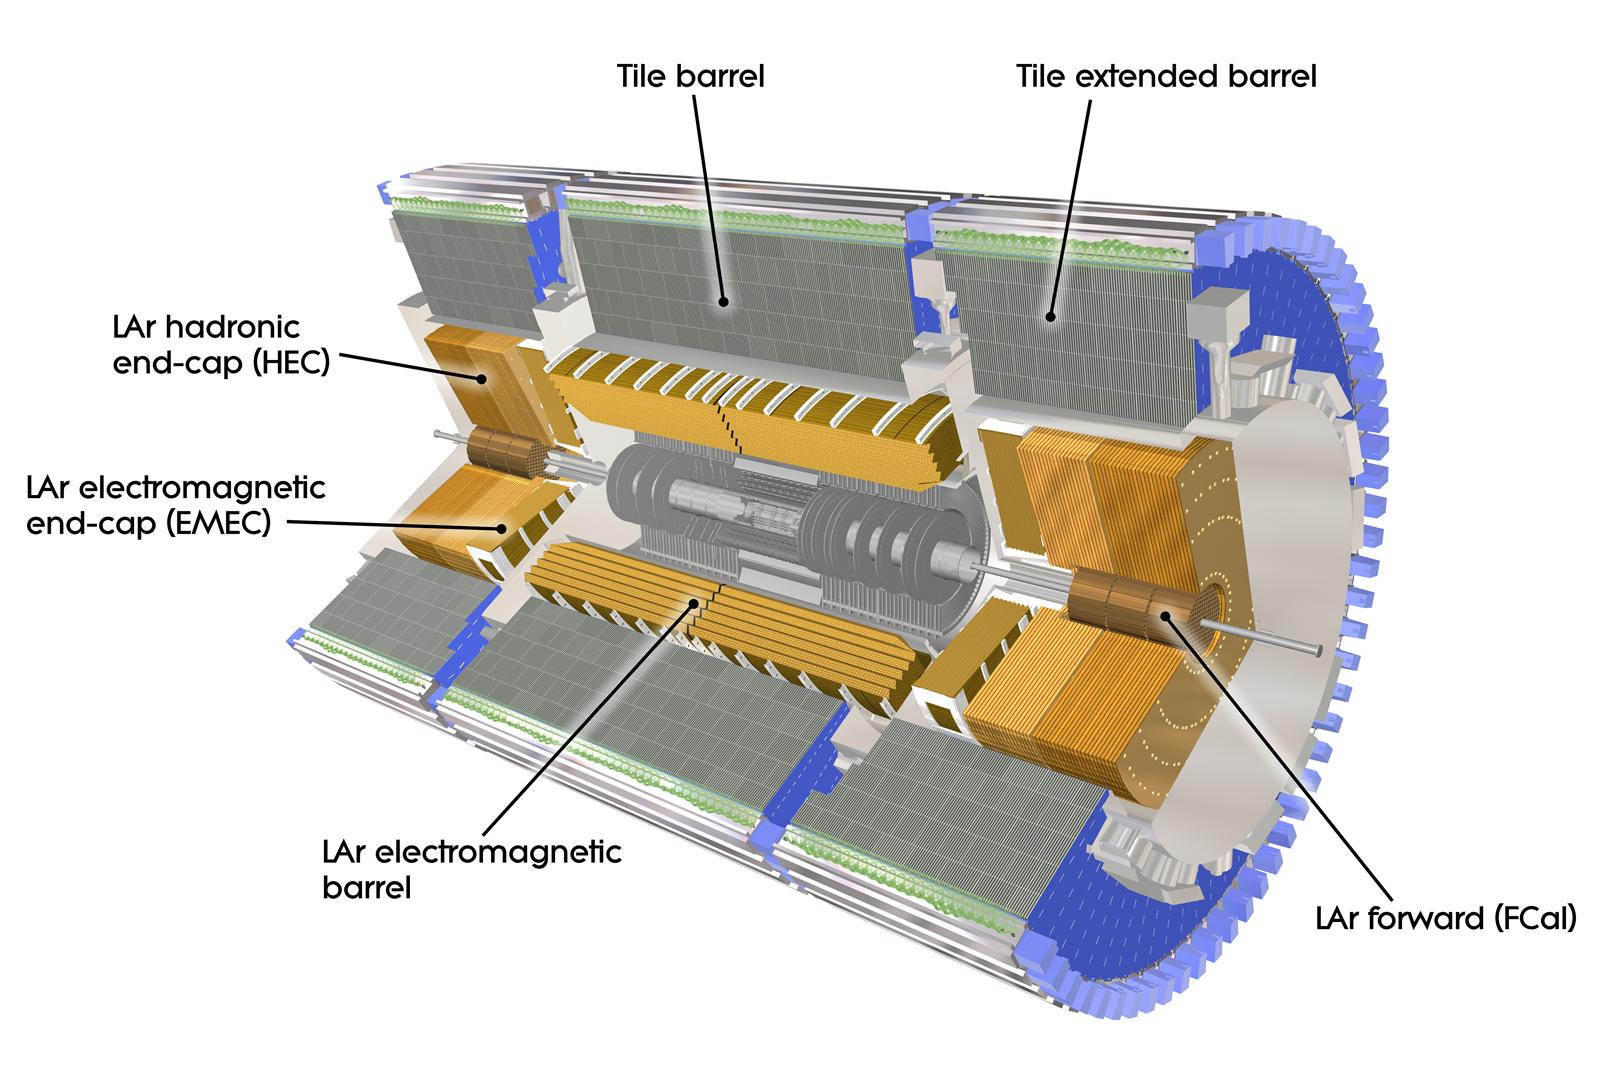
\includegraphics[height=7cm,keepaspectratio]{calocalo.jpg}
  \caption[ATLASカロリメータ]{カロリメータの全体図 \cite{calocalo} }
  \label{fig:calocalo}
\end{figure}

\fref{fig:calocalo}にカロリメータの全体像を示す。ATLASにおけるカロリメータはサンプリング型のカロリメータであり、検出層と吸収層から成る積層構造である。カロリメータは内部飛跡検出器の外側に配置されており、全体で$|\eta|<4.9$の領域を覆うように配置されている。粒子と物質の相互作用の違いから、対象とする粒子の種類により電磁カロリメータとハドロンカロリメータが用意されている。このような構造から、カロリメータを用いて通過粒子のエネルギーや位置の測定、電子・光子とハドロンの区別、ジェットの識別を行うことができる。

電磁カロリメータは、ソレノイド磁石の外側のバレル部($|\eta|<1.4$)とエンドキャップ部($1.4<|\eta|<3.2$)の領域に設置されている。検出層に液体アルゴン\footnote{液体アルゴン(LAr)はエネルギー応答が線形で且つ安定を持つ物質である。また、放射線耐性も充分持ち合わせている。}、吸収層に鉛($\mathrm{Z}=82$)が用いられており、高エネルギーの電子・光子が電磁カロリメータに到達すると、吸収層において電子対生成や制動放射を繰り返し、電磁シャワーを形成する。低エネルギーになった粒子は検出層においてイオン化しエネルギーを失い、イオン化により発生した電子が電気信号として読み出される。電磁シャワーによって得られる合計エネルギーを計算することにより、入射電子・光子のエネルギー測定を行うことができる。電子と光子の区別は、内部飛跡検出器中の飛跡情報を用いて行う。
電磁カロリメータの厚さは$20X_0$\footnote{$X_0$は放射長であり、入射粒子のエネルギーが$1/e\sim0.37$となる距離である。}を超えるため、測定対象である電子・光子のほとんどは電磁カロリメータにおいて全てのエネルギーを失う。

ハドロンカロリメータは、電磁カロリメータの外側にあり、バレル部($|\eta|<1.7$)とエンドキャップ部($1.5<|\eta|<3.2$)の領域に設置されている。バレル部は検出層にシンチレータ、吸収体に鉄を用いたタイルカロリメータから成り、エンドキャップ部では検出層に液体アルゴン、吸収層に銅が用いられる。高エネルギーのハドロンがハドロンカロリメータに入ると、吸収層において原子核と強い相互作用し粒子多重生成を行い、カスケードシャワーを発生しそのエネルギー測定を行う。



%------------------------------------------------------------------------------------------------------------------------
\subsection{ミューオン検出器}
\label{sec:mumu}
%------------------------------------------------------------------------------------------------------------------------
ミューオン検出器はカロリメータの外側にあり、$|\eta|<2.7$の領域に設置される、ATLASにおける最外層の検出器である。ミューオンは物質の透過力が高く、他の崩壊生成粒子と比較して寿命が長い($\sim 2.2\ \si{\micro sec}$)ため、ATLASの外側まで透過する。予想される最高エネルギー($1\ \si{TeV}$)までのミューオンの運動量を測定できるよう設計されている。

ミューオン検出器の大部分は、MDT(\textbf{M}onitored \textbf{D}rift \textbf{T}ube)である。MDTは直径約$3\ \si{cm}$のドリフトチューブ検出器であり、ミューオンの通過位置を測定することができる。測定のトリガーとして、バレル部においてはRPC(\textbf{R}esistive \textbf{P}late \textbf{C}hamber)、エンドキャップ部においてはTGC(\textbf{T}hin \textbf{G}ap \textbf{C}hamber)から得られる情報を用いる。ビームパイプに近い領域($2.0<|\eta|<2.7$)においては、バックグラウンドの$\gamma$線や中性子が多く,ヒットレートが大きい。MDTはドリフト時間が長いため、この領域においてはMDTではなく高い入射レートに耐えられるCSC(\textbf{C}athode \textbf{S}trip \textbf{C}hamber)を用いてミューオンの通過位置測定を行う。







%------------------------------------------------------------------------------------------------------------------------
\section{HL-LHCアップグレード}
\label{sec:HL-LHC}
%------------------------------------------------------------------------------------------------------------------------
\begin{figure}[tbp]
  \centering
  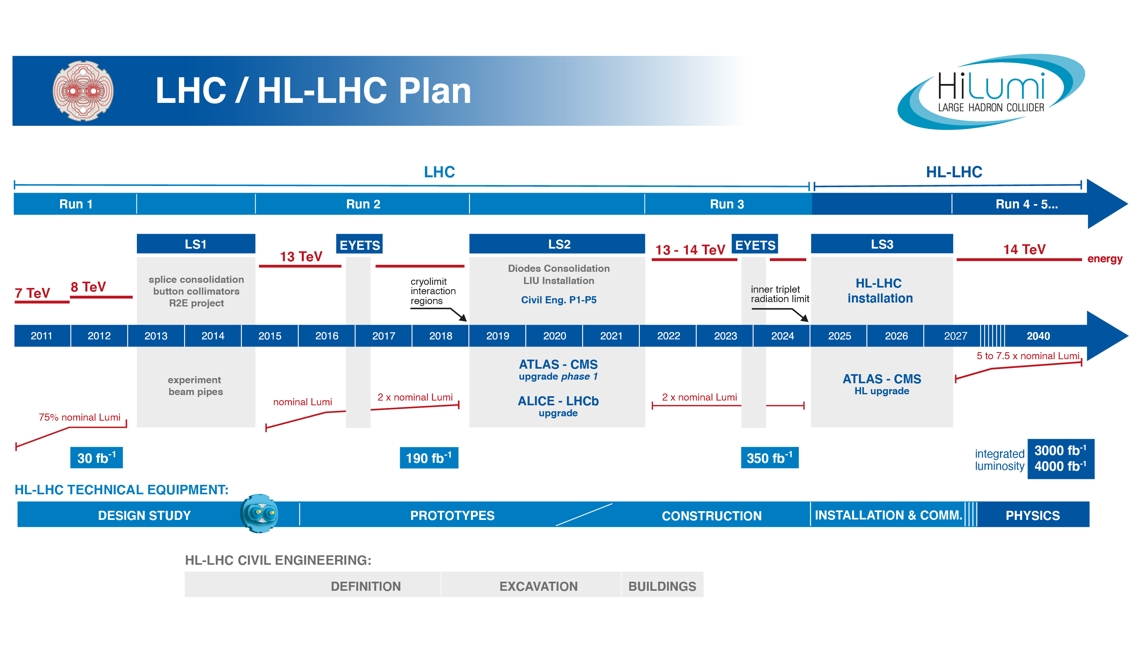
\includegraphics[height=8cm,keepaspectratio]{HL-LHC-January-2021_small.jpg}
  \caption[LHCの運転計画]{2021年1月に作成されたLHCの運転計画 \cite{hl-lhc}。2025年 }
  \label{fig:hl-lhc}
\end{figure}

\fref{fig:hl-lhc}にLHCの運転計画を示す。LHCでは、2025年から\textbf{HL-LHC}(High Luminosity LHC)アップグレードが開始する予定である。2027年の運転開始から瞬間ルミノシティを設計値である$1.0\times 10^{34}\ \si{cm^{-2}s^{-1}}$の$5 \mathchar`- 7$倍に増加させ、2037年における運転停止までの積分ルミノシティをRun3までで取得予定である$300\ \si{fb^{-1}}$の約$10$倍にまで増加させることが目標である。

このアップグレードに伴い、ATLASに配置される検出器についてもアップグレードが予定されている。この節では、HL-LHCアップグレード計画と、本研究と関わりのあるATLAS内部飛跡検出器のアップグレード計画について述べる。

%------------------------------------------------------------------------------------------------------------------------
\subsection{HL-LHCの概要}
\label{sec:HL-LHC-gaiyou}
%------------------------------------------------------------------------------------------------------------------------
%\begin{figure}[tbp]
%  \centering
%  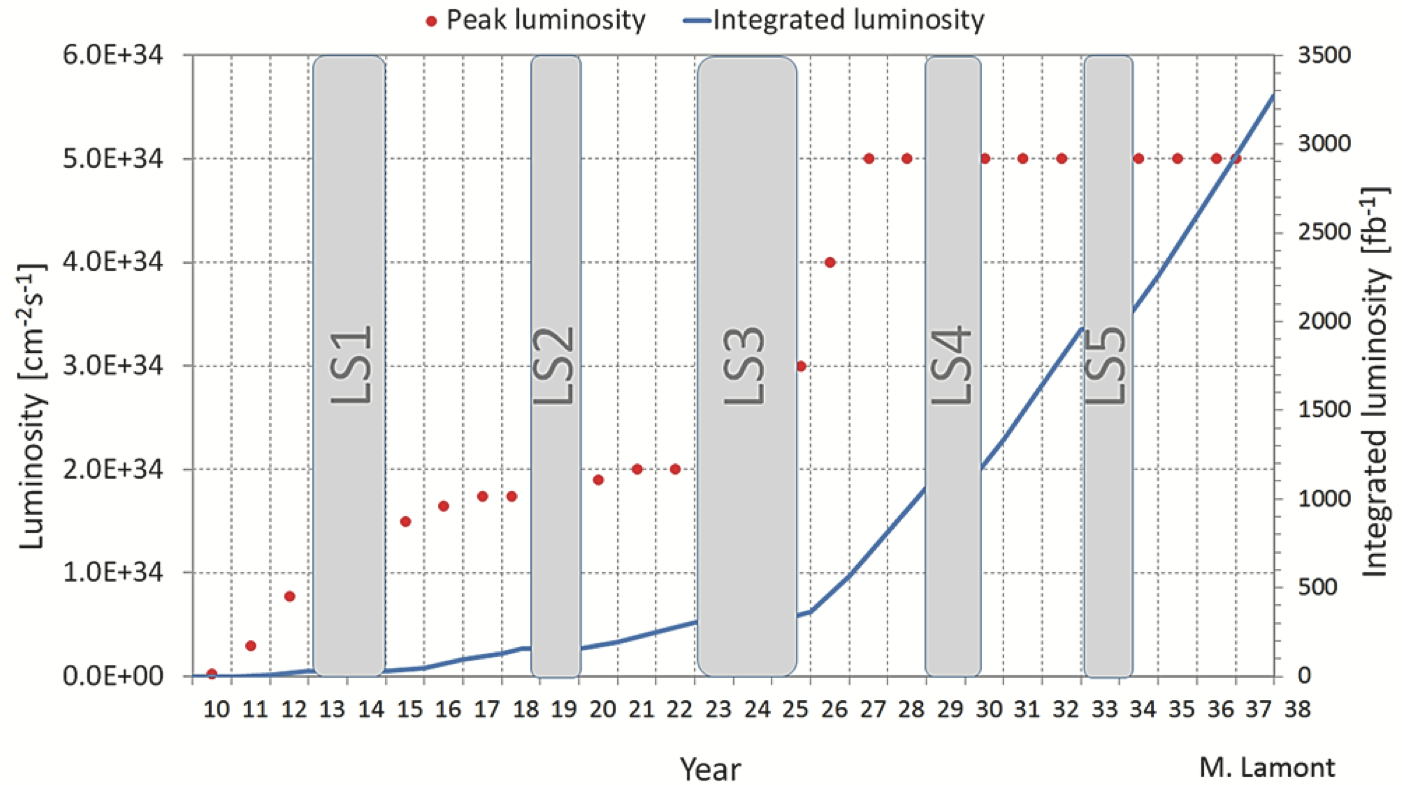
\includegraphics[height=7cm,keepaspectratio]{time_lumi.png}
%  \caption[LHCのピークルミノシティと積分ルミノシティ]{ \cite{lhc-lumi}}
%  \label{fig:time-lumi}
%\end{figure}

\begin{table}[htbp]
  \begin{center}
    \caption[HL-LHCでのビームパラメータ]{HL-LHCでのビームパラメータ\cite{lhc-lumi}}
    \label{tab:genkou-hl}
    \begin{tabular}{|l||c|c|}
    \hline
      パラメータ & 現行LHC & HL-LHC \\
    \bhline{1.5pt}
    陽子エネルギー [\si{TeV}] & 7 & 7 \\
    \hline
    1バンチあたりの陽子数 $N_b$ & $1.15\times 10^{11}$ & $2.2\times 10^{11}$ \\
    \hline
    交差角$\theta_c\ [\si{\micro rad}]$ & 285 & 590 \\
    \hline
    幾何学的損失係数$R$(括弧内はクラブ空洞無し) & 0.836 & 0.829 (0.305) \\
    \hline
    衝突点における振幅$\beta^*\ [\si{m}]$ & 285 & 590 \\
    \hline
    $xy$平面のビームの広がり$\varepsilon_n\ [\si{\micro m}]$ & 3.75 & 2.50 \\
    \hline
    1交差あたりの事象数(パイルアップ) & 27 & 138 \\
    \hline
    パイルアップ密度[$\si{/mm}$] & 0.21 & 1.25 \\
    \hline
    積分ルミノシティ[$\si{fb^{-1} /year}$] & 45 & 260 \\
    \hline
    \end{tabular}
  \end{center}
\end{table}

LHCは2010年春から本格運転を開始し、長期運転停止期間(LS: \textbf{L}ong \textbf{S}hutdown)を重ねて、ピークルミノシティを設計値である$1.0\times 10^{34}\ \si{cm^{-2}s^{-1}}$の$2$倍まで向上させ、データ取得を行っていく予定である。さらに、2025年-2027年における長期運転停止期間(LS3)においてLHCのアップグレードを行い、瞬間ルミノシティを現行LHCの設計値の$5 \mathchar`- 7$倍にまで増加させる。

\tref{tab:genkou-hl}に現行LHCとHL-LHCで予定されている主なビームパラメータをまとめる。
\eref{eq:lumi}より、瞬間ルミノシティを増大させるには、ビーム電流($N_b, n_b$)を増強し、衝突点でのビームサイズ($\varepsilon_n, \beta^*$)を絞り、交差角$\theta_c$による幾何学的損失係数$R$をできるだけ大きくするよう設計する必要がある。そのため、HL-LHCではルミノシティを大幅に向上させるために以下のような改良を計画している。
\begin{itemize}
  \item LHCに入射する陽子ビームの強度と輝度を向上させるため、前段加速器の各機器(Linac4, PSB, PS, SPS)について更新・アップグレードを実施
  \item 衝突点でのビームサイズを絞る(衝突点における振幅$\beta^*$を減少)ため、ATLAS、CMSの衝突点周りの挿入部に新たに高磁場の磁石を実装
  \item 幾何学的損失係数$R$を現行LHCと同程度に保つため、衝突点のクラブ空洞\footnote{「クラブ空洞」とは、高エネルギー加速器研究機構(KEK)で開発された特殊な超伝導空洞で、電子・陽電子ビームのバンチを回転させることにより、より高いルミノシティを達成することを目指して開発された技術である。\cite{crab}}を導入
\end{itemize}






%------------------------------------------------------------------------------------------------------------------------
\subsection{内部飛跡検出器のアップグレード}
\label{sec:hl-lhc-itk}
%------------------------------------------------------------------------------------------------------------------------
HL-LHCにおいて、ATLASはこれまでよりもさらに過酷な放射線環境下に晒される。瞬間ルミノシティが現行LHCの設計値の$5 \mathchar`- 7$倍にまで増加するため、現行のATLASを用いてHL-LHCの環境下において測定を行うと主に二つの問題が生じると予想される。
\begin{itemize}
\item 瞬間ルミノシティが大きくなることにより、バンチ衝突あたりの生成粒子数が増加し放射線損傷の影響がより大きくなる。検出器のセンサーが放射線損傷を受けると、検出効率が低下するため、より高い放射線耐性を持つ検出器が要求される。
\item 各検出器のヒット占有率の増加である。HL-LHCでは、パイルアップが$200$まで増加すると予想されており内部飛跡検出器での飛跡の数が増加することで、飛跡の識別が困難になり、再構成の性能が大幅に低下する。特に、荷電粒子への感度が高いガス検出器であるTRTでは検出器の占有率が$100\si{\%}$に達してしまうと予想されている。そのため、HL-LHCにおいてはよりパイルアップ耐性が高い検出器が必要となる。
\end{itemize}
%これらの問題により、ピクセル検出器に対する要求は\tref{tab:hlVSIBL}となっている。放射線耐性について$1\ \si{MeV}$の中性子換算で$1.4\times 10^{16}\ \si{n_{eq}/cm^2}$という。また、位置分解能向上およびヒット占有率の増加を防ぐため、ピクセルサイズは現行IBLの$1/5$になっている。

\begin{table}[htbp]
  \begin{center}
    \caption[HL-LHCでのビームパラメータ]{HL-LHCでのビームパラメータ\cite{lhc-lumi}}
    \label{tab:genkou-hl}
    \begin{tabular}{|l||c|c|}
    \hline
      パラメータ & 現行IBL & ITk \\
    \bhline{1.5pt}
    ピクセルサイズ [$\si{\micro m^2}$] & 7 & 7 \\
    \hline
    読み出しデータレート $N_b$ & $1.15\times 10^{11}$ & $2.2\times 10^{11}$ \\
    \hline
    交差角$\theta_c\ [\si{\micro rad}]$ & 285 & 590 \\
    \hline
    幾何学的損失係数$R$(括弧内はクラブ空洞無し) & 0.836 & 0.829 (0.305) \\
    \hline
    衝突点における振幅$\beta^*\ [\si{m}]$ & 285 & 590 \\
    \hline
    $xy$平面のビームの広がり$\varepsilon_n\ [\si{\micro m}]$ & 3.75 & 2.50 \\
    \hline
    1交差あたりの事象数(パイルアップ) & 27 & 138 \\
    \hline
    パイルアップ密度[$\si{/mm}$] & 0.21 & 1.25 \\
    \hline
    積分ルミノシティ[$\si{fb^{-1} /year}$] & 45 & 260 \\
    \hline
    \end{tabular}
  \end{center}
\end{table}


\begin{figure}[tbp]
  \centering
  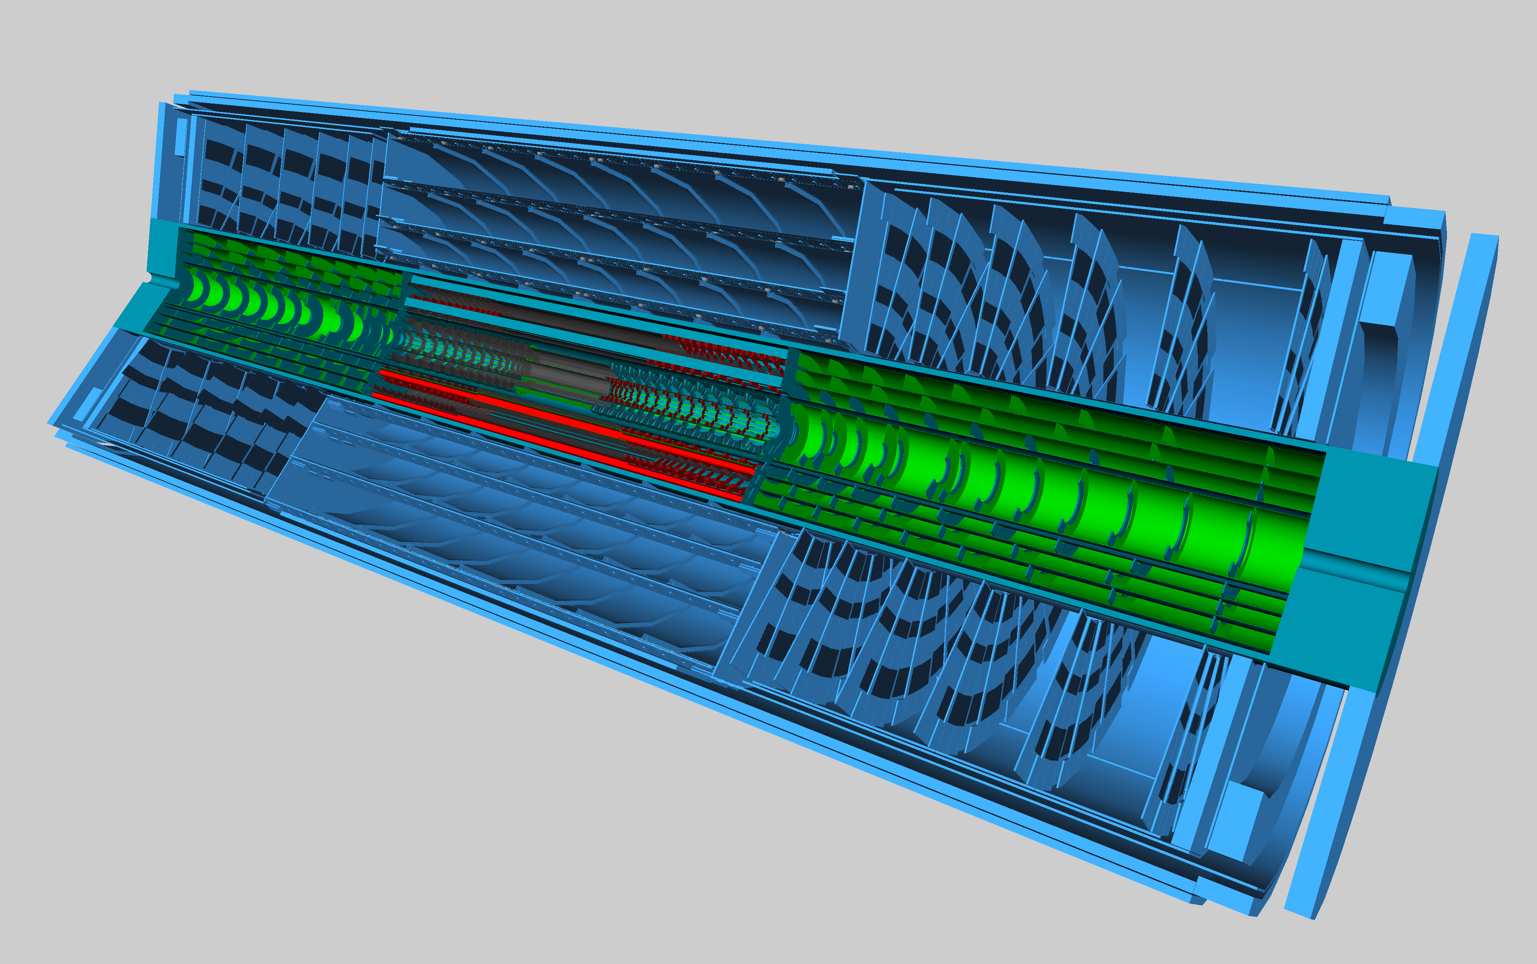
\includegraphics[height=8cm,keepaspectratio]{itk_display.png}
  \caption[ITkの断面図]{ITkの断面図 \cite{itk}。}
  \label{fig:hl-lhc-itk}
\end{figure}

\begin{figure}[tbp]
  \centering
  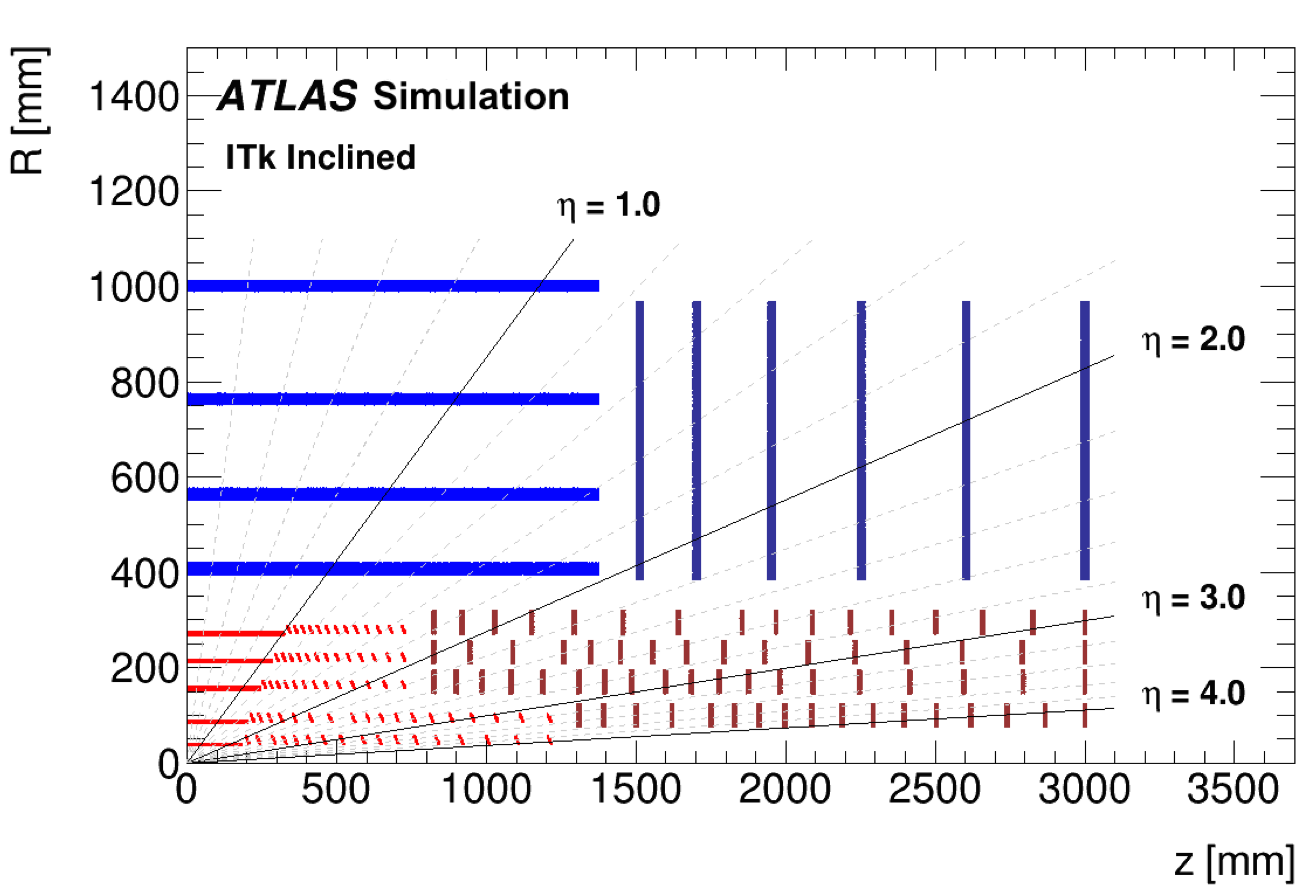
\includegraphics[height=8cm,keepaspectratio]{atlas_itk.png}
  \caption[ITkの断面図]{ITkの断面図 \cite{itk}。}
  \label{fig:itk-danmen}
\end{figure}

以上の理由により、ATLASの衝突点に最も近い検出器である内部飛跡検出器の総入れ替えを計画している。HL-LHCのために開発されている、新たな内部飛跡検出器を\textbf{ITk}(\textbf{I}nner \textbf{T}rac\textbf{k}er)と呼ぶ。
ITkの全体像を\fref{fig:hl-lhc-itk}に示す。ITkは全てシリコン半導体検出器から構成され、\fref{fig:itk-danmen}に示すように、TRTは廃止されて、内側にピクセル検出器、外側にストリップ検出器が配置されている。
%ピクセル検出器はバレル部の5層とエンドキャップ部の 層、ストリップ検出器はバレル部の4層とエンドキャップ部の6層から構成され、ITk全体で$|\eta|<4$の領域を覆うように配置されている。

上で挙げた、放射線損傷についての問題を解消するために、ピクセル検出器に新たな半導体センサーを導入する。特に、放射線の影響が大きくなるバレル部の最内層では高放射線耐性を持つ3Dセンサーを使用することが予定されている。ヒット占有率の問題については、センサーの厚みを薄くし、ピクセルサイズを現行ピクセルの$1/5$にすることにより、ヒット占有率を抑えることが期待される。さらに、1衝突あたりのパイルアップが高くなることから、読み出しシステムの高速化も必要となる。


このようなアップグレードを行うことにより、HL-LHCにおける高い瞬間ルミノシティ環境下においても、高い飛跡再構成効率における解析を行うことができる。
さらに、現行LHCの検出範囲外であった$2.7<|\eta|$が検出可能になることにより、フェイクレートを抑えつつ、$3\ \si{GeV}$以上のミューオンを$99\si{\%}$以上の効率で検出、さらには$1\ \si{GeV}$以上の電子やパイオンを$85\si{\%}$以上の効率で検出可能となる。



%------------------------------------------------------------------------------------------------------------------------
\subsection{HL-LHC physics}
\label{sec:hl-lhc-physics}
%------------------------------------------------------------------------------------------------------------------------

%素粒子のところと内容を合わせる。
%統計量がどれくらい必要で、それが再現できる?

%\fref{fig:hl-lhc}にある運転計画のように、LHCでは2010年の運転開始から統計をため、積分ルミノシティはRUN1の終了時において$30\ \si{fb^{-1}}$、RUN2の終了時において$190\ \si{fb^{-1}}$となっている。



\newpage
